%!TEX program = xelatex
\documentclass{article}
\usepackage{amsthm,amsmath,amssymb}
\usepackage[UTF8]{ctex}
\usepackage[tc]{titlepic}
\usepackage{titlesec}
\usepackage{cite}
\usepackage{fancyhdr}
\usepackage{booktabs}
\usepackage{graphicx}
\usepackage{subfigure}
\usepackage{float}
\usepackage{geometry}
\usepackage[section]{placeins}
\usepackage{makeidx}
\usepackage{mathrsfs}
\usepackage{color}
\usepackage{ulem}
\usepackage{enumitem}
\everymath{\displaystyle}
\geometry{a4paper,scale=0.8}
\pagestyle{fancy}

\usepackage{hyperref}
\hypersetup{hypertex=true, colorlinks=true, linkcolor=blue, anchorcolor=blue, citecolor=blue}

\usepackage{listings}
\lstset{
    language=Python,
    basicstyle=\small\ttfamily,
    keywordstyle=\color{blue},
    commentstyle=\color{green},
    stringstyle=\color{red},
    showstringspaces=false,
    breaklines=true,
}

\lhead{第 3 次作业\\\today}
\chead{中国科学技术大学\\	DS4001 人工智能原理与技术}

\rhead{Homework 3\\ {\CTEXoptions[today=old]\today}}
\newcommand{\upcite}[1]{\textsuperscript{\cite{#1}}}

\titleformat*{\section}{\bfseries\Large}
\titleformat*{\subsection}{\bfseries\large}

\title{\bfseries 第三次作业(贝叶斯网络)}
\author{崔士强  \quad  PB22151743}

\begin{document}
\maketitle
% \clearpage

\section*{问题1:概率推断}
\subsection*{a.}
\begin{figure}[H]
    \centering
    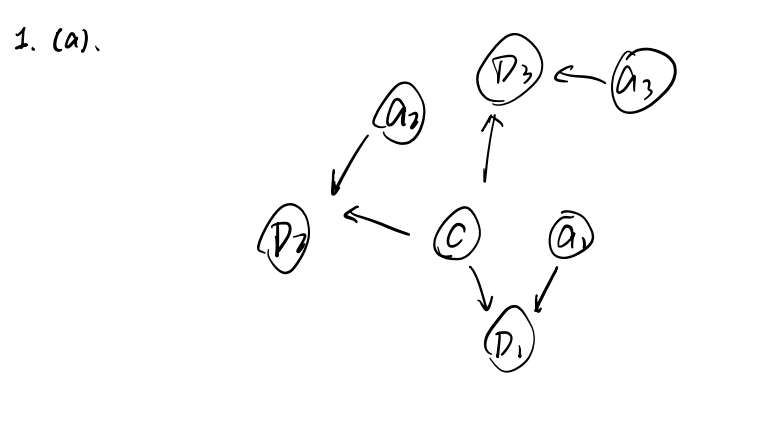
\includegraphics[scale=0.5]{1a.png}
\end{figure}
\subsection*{b.}
\begin{figure}[H]
    \centering
    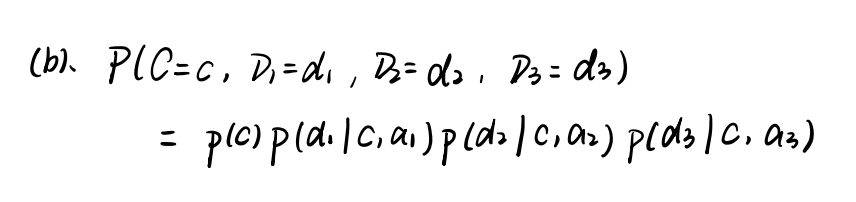
\includegraphics[scale=0.5]{1b.png}
\end{figure}
\subsection*{c.}
\begin{figure}[H]
    \centering
    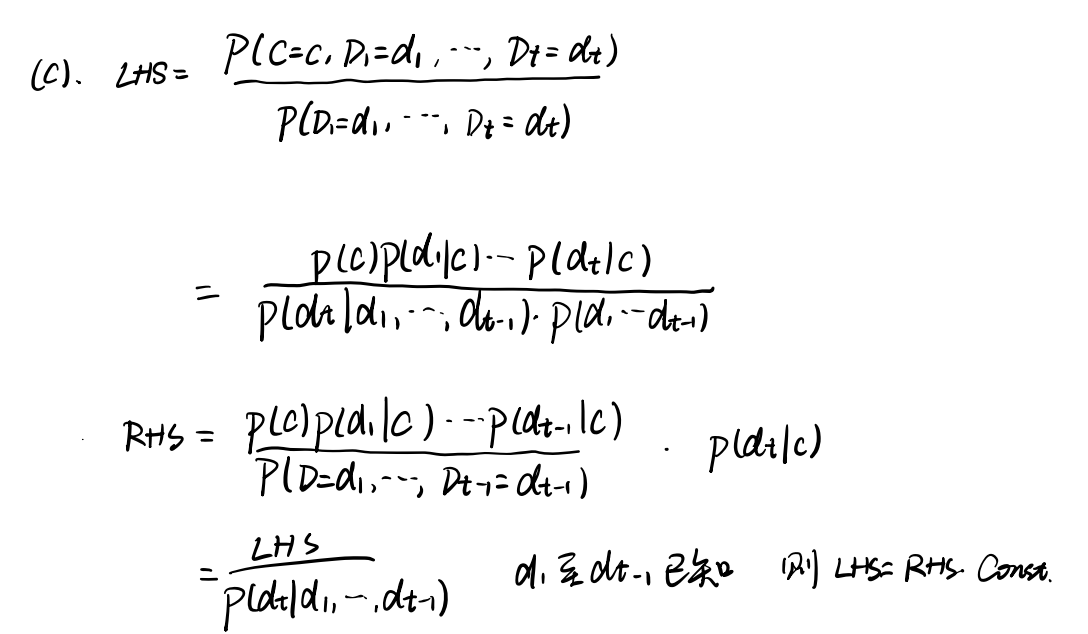
\includegraphics[scale=0.5]{1c.png}
\end{figure}
\subsection*{d.}
\begin{lstlisting}
    def observe(self, agentX: int, agentY: int, observedDist: float) -> None:
        # BEGIN_YOUR_CODE (our solution is 7 lines of code, but don't worry if you deviate from this)
        for row in range(self.belief.numRows):
            for col in range(self.belief.numCols):
                prob = self.belief.getProb(row, col)    # Probability at current index
                targetX, targetY = util.colToX(col), util.rowToY(row)   # Get location of current index
                distance = math.sqrt(math.pow(agentX-targetX, 2)+math.pow(agentY-targetY, 2))
                multiplier = util.pdf(distance, Const.SONAR_STD, observedDist)
                self.belief.setProb(row, col, prob*multiplier)
        self.belief.normalize()
        # END_YOUR_CODE
\end{lstlisting}

\section*{问题2:转移概率}
\subsection*{a.}
\begin{figure}[H]
    \centering
    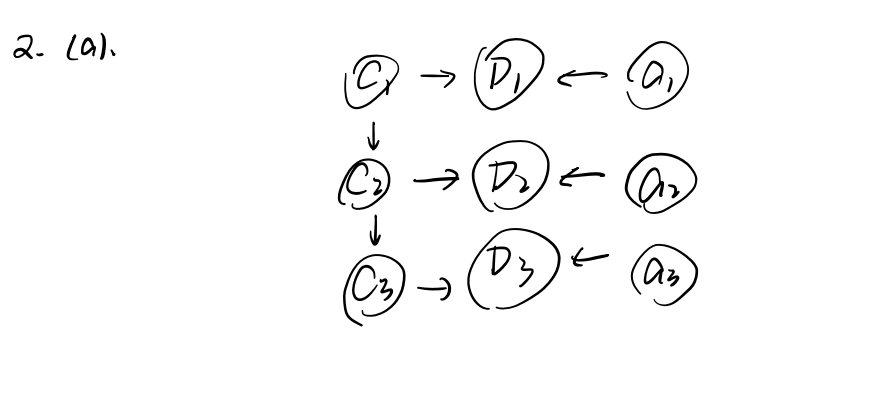
\includegraphics[scale=0.5]{2a.png}
\end{figure}
\subsection*{b.}
\begin{figure}[H]
    \centering
    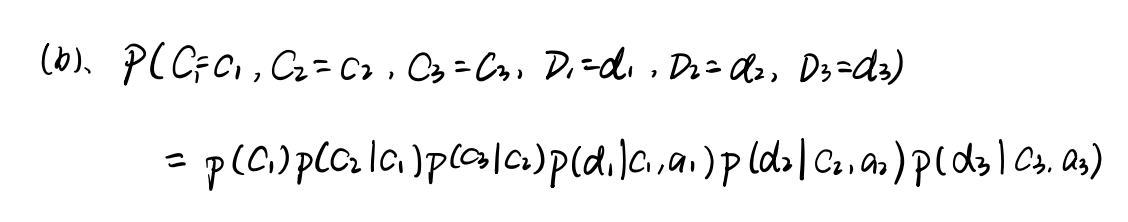
\includegraphics[scale=0.5]{2b.png}
\end{figure}
\subsection*{c.}
\begin{figure}[H]
    \centering
    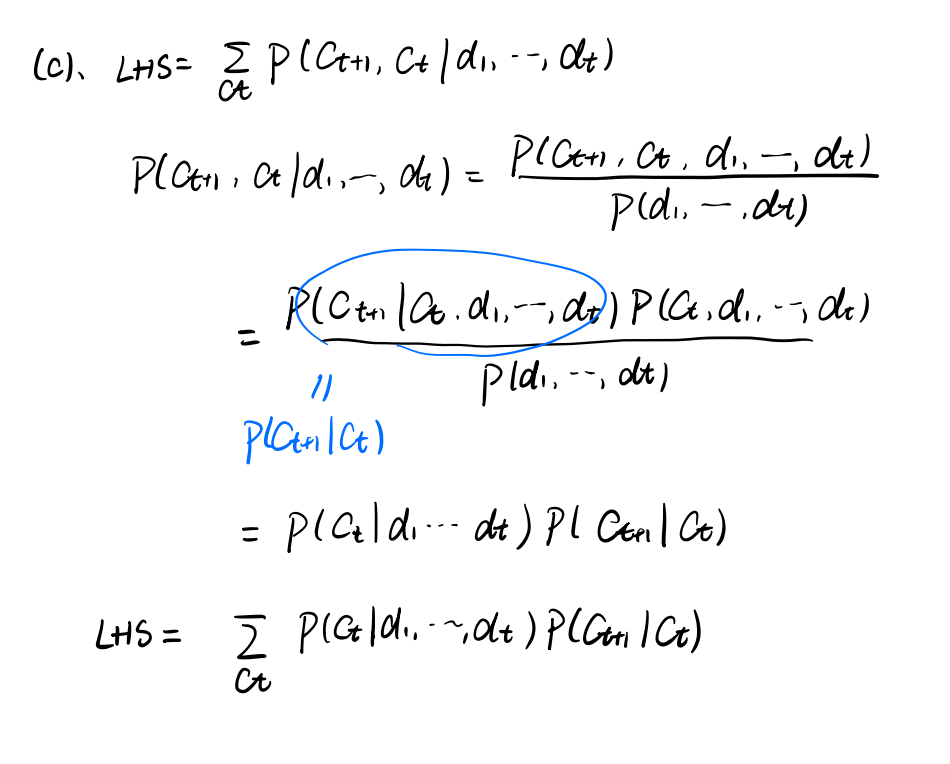
\includegraphics[scale=0.5]{2c.png}
\end{figure}
\subsection*{d.}
\begin{lstlisting}
    def elapseTime(self) -> None:
        if self.skipElapse: ### ONLY FOR THE GRADER TO USE IN Problem 1
            return
        # BEGIN_YOUR_CODE (our solution is 7 lines of code, but don't worry if you deviate from this)
        temp_belief = self.belief
        for row in range(self.belief.numRows):
            for col in range(self.belief.numCols):
                prob = 0.0
                for key in self.transProb:
                    if key[1] == (row, col):
                        prob += self.belief.getProb(key[0][0], key[0][1])*self.transProb[key]
                temp_belief.setProb(row, col, prob)
        temp_belief.normalize()
        self.belief = temp_belief
        # END_YOUR_CODE
\end{lstlisting}


\section*{问题3:是哪辆车?}
\subsection*{a.}
\begin{figure}[H]
    \centering
    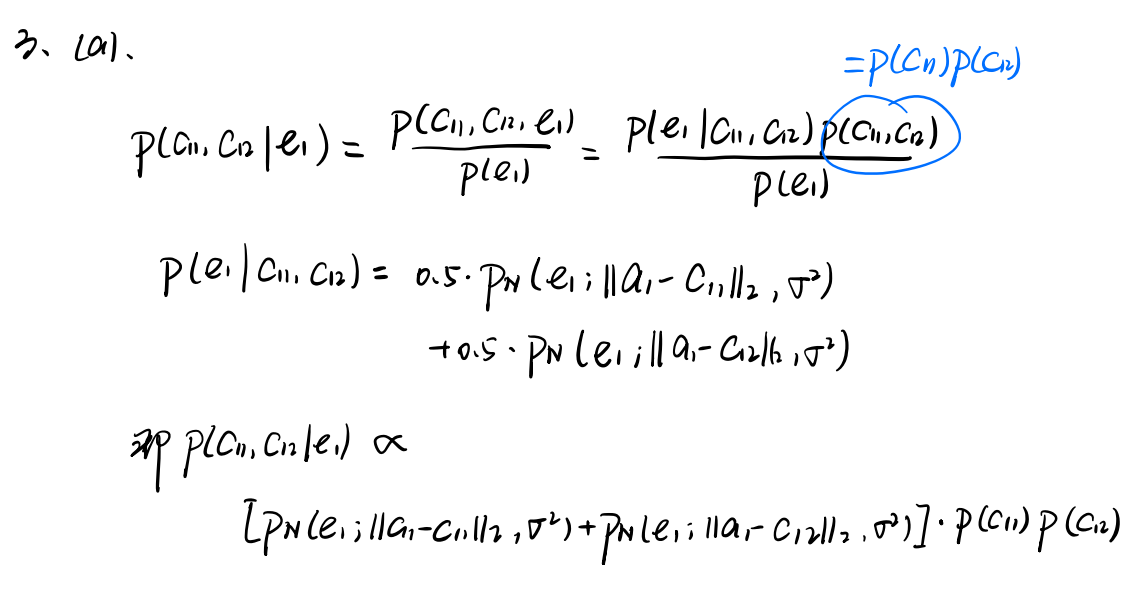
\includegraphics[scale=0.5]{3a.png}
\end{figure}
\subsection*{b.}
\begin{figure}[H]
    \centering
    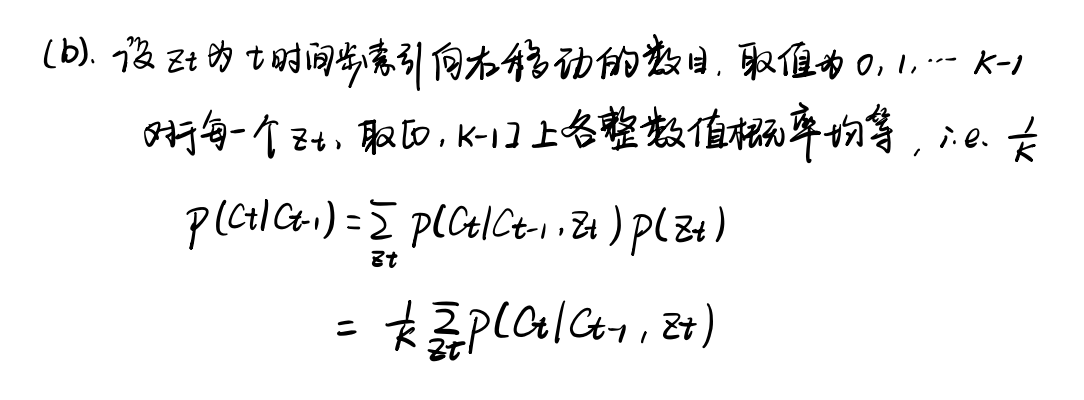
\includegraphics[scale=0.5]{3b.png}
\end{figure}
\subsection*{c.}
\begin{figure}[H]
    \centering
    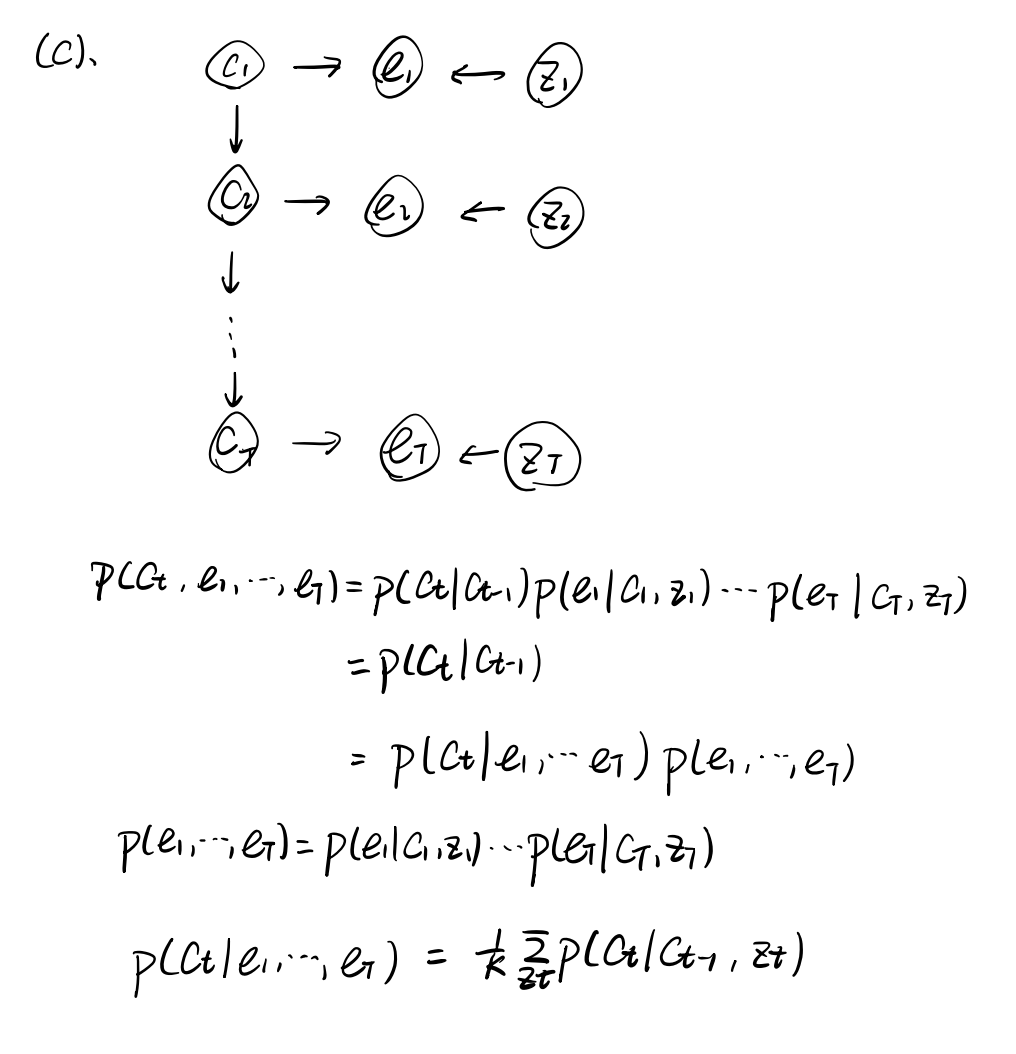
\includegraphics[scale=0.5]{3c.png}
\end{figure}
\subsection*{d.}
粒子滤波相比精确推理,速度上有明显的提升,另外成功率也有显著改善,在车辆数增加的情况下也是如此。

原因是精确推理需要存储整个空间上的概率分布,导致计算的复杂度很高。而粒子滤波使用一组有限数量的粒子,计算复杂度主要取决于粒子的数量而非状态空间。
\section*{问题4:模型学习}
\subsection*{a.}
\begin{figure}[H]
    \centering
    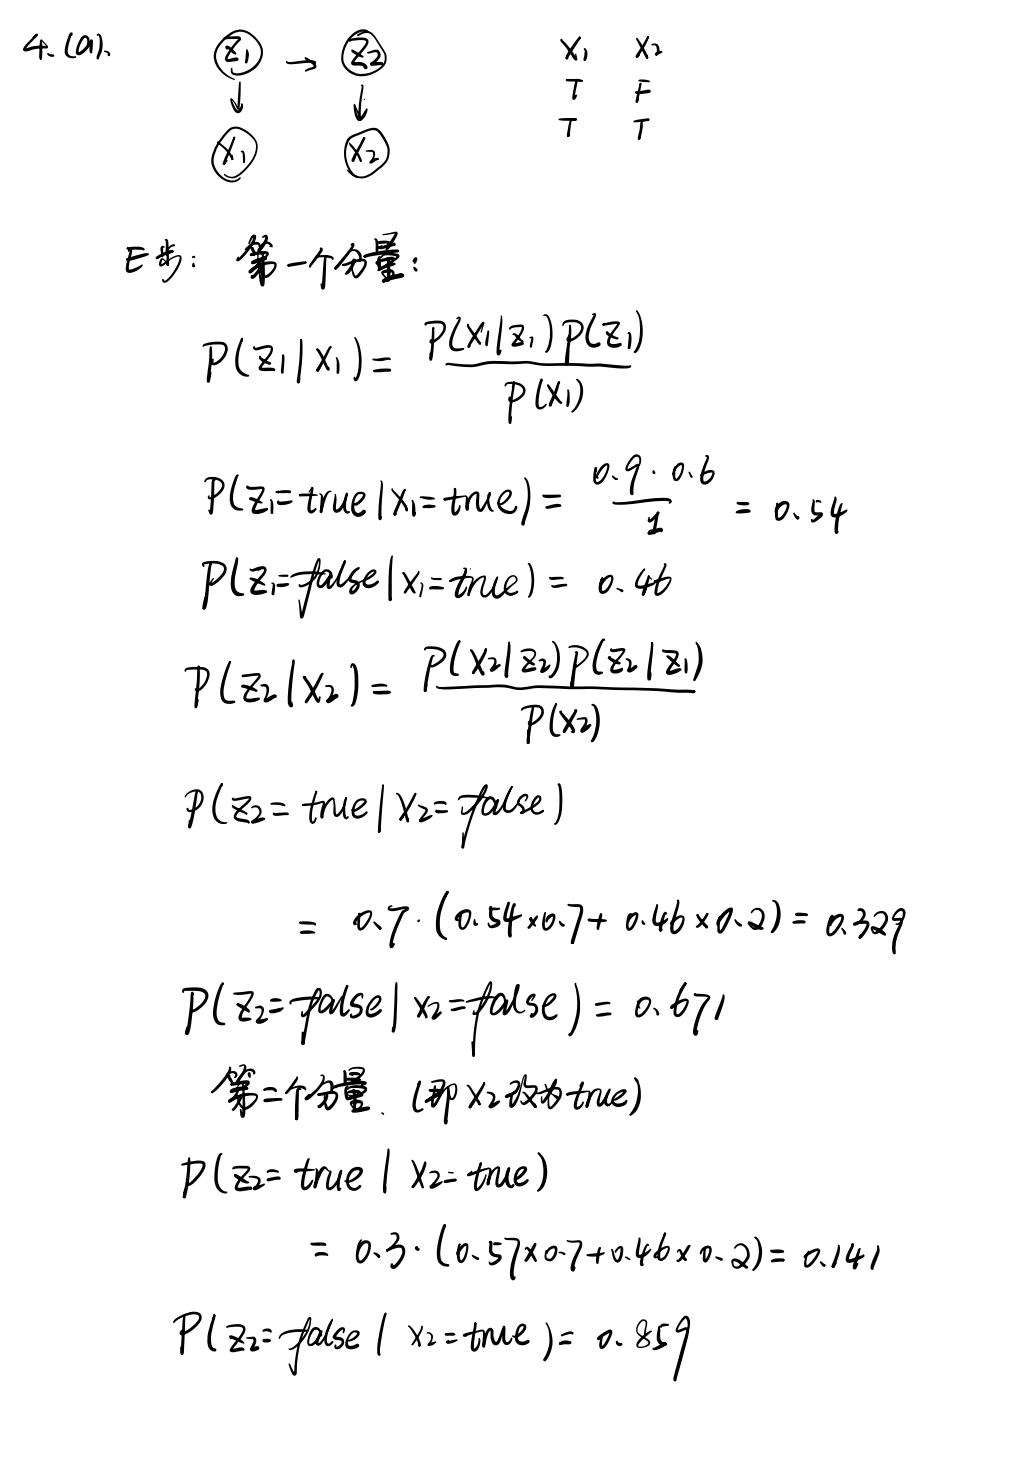
\includegraphics[scale=0.5]{4a.png}
\end{figure}
\section*{反馈}
% 在每次实验报告的最后欢迎反馈你上这门课的感受,你可以写下任何反馈,包括但不限于以下几个方面:课堂、作业难度和工作量、助教工作等等。

\begin{itemize}
    \item 代码部分没有难度,书写部分3,4题感觉有些难度,无论是在理解题意上还是在解题上。
    \item 整体用时在20h左右,大部分是在做计算以及证明题。
\end{itemize}

\end{document}